
\chapter{Ising模型}
\section{Ising模型と熱統計力学の基礎}
強磁性体を記述するモデルのひとつ.
\subsection{ハミルトニアン}
ハミルトニアンを
\begin{eqnarray}
  H = -J\sum_{\ev{i, j}}s_i\cdot s_j
\end{eqnarray}
とする. $\ev{i, j}$は隣接サイト間のみの和を表す. $J$は相互作用定数. $s$はスピン. スピンはアップ($s = 1$)とダウン($s = -1$)の2種類. 非常に単純なスピン系モデルでありながら相転移の記述が可能である. 1・2次元系については厳密解が求められている.

外部磁場を考慮したモデルもある:
\begin{eqnarray}
  H = -J\sum_{\ev{i, j}}s_i\cdot s_j -h\sum_i s_i\label{Ising2}
\end{eqnarray}

\subsection{平衡状態}
系の平衡状態はHelmholtzエネルギー
\begin{eqnarray}
  F = U -TS
\end{eqnarray}
が最小になるように決まる. 低温 ($T \ll U/S$)ならば内部エネルギー $U = \ev{H}$ がleading であり, これを最小化するようにスピンの向きが揃う. これを強磁性体と呼ぶ. 一方で高温ならばエントロピーの項が優勢なのでエントロピーが最大になるようにスピンの向きがバラバラになる. これを常磁性体と呼ぶ.

\subsection{相転移}
Gibbs自由エネルギーの1回微分が不連続変化をするときこれを第一種相転移と呼び, Gibbs自由エネルギーの2回微分については第二種相転移と呼ぶ. 第一種は体積, エントロピーとか. 
\begin{eqnarray}
  \qty(\frac{\partial G}{\partial p})_T = V, \hspace{1cm} \qty(\frac{\partial G}{\partial T})_p = -S
\end{eqnarray}
第二種は比熱など.
\begin{eqnarray}
\frac{\partial^2 G}{\partial T^2} = -\frac{\partial S}{\partial T} = -\frac{C_P}{T}
\end{eqnarray}
有限温度1次元Ising模型は相転移を起こさないが, 2次元系はその限りではない.

\section{Ising模型の厳密解}
\subsection{1次元Ising模型 : 平均場近似}
まずは厳密解の前にIsing模型を平均場近似で解析してみる. 多体系で相互作用を平均場として理解することは非常に重要なので, 手法として知っておく必要がある.

平均場近似ではまず任意のサイトのスピンに着目し, その周囲のスピンからの影響を時間や空間によらない平均値で置き換える. スピンを
\begin{eqnarray}
  s_i = \ev{s} + \delta s_i
\end{eqnarray}
置くことにする. これを(\ref{Ising2})に代入:
\begin{eqnarray}
  H &=& -H_{\rm{eff}}\sum_{i=1}^N s_i + \frac{NzJ\ev{s}^2}{2}\\
  H_{\rm{eff}} &=&  h + zJ\ev{s}
\end{eqnarray}
ここで$\delta s$の2次は無視している. $N$はスピンの総数, $z$は最隣接サイト数(1次元なら2, 2次元なら4)である. 計算途中で
\begin{eqnarray}
  \sum_{\ev{i, j}}s_i = z\sum_i s_i, \hspace{0.5cm}\sum_{\ev{i, j}}1 = \frac{1}{2}zN
\end{eqnarray}
を用いている. これより分配関数は
\begin{eqnarray}
  Z &=& \exp\qty(-\beta H) = \exp\qty[-\beta\qty(-H_{\rm{eff}}\sum_{i=1}^N s_i + \frac{NzJ\ev{s}^2}{2})] = Z_0\qty(\prod_iZ_i) = Z_0(Z_i)^N\\
  Z_0 &=& \exp\qty(-\beta\frac{NzJ\ev{s}^2}{2}), \hspace{0.5cm}Z_i = \sum_{s_i = 1, -1}e^{\beta H_{\rm{eff}}s_i} = 2\cosh\qty(\beta H_{\rm{eff}})
\end{eqnarray}
全体の分配関数は
\begin{eqnarray}
  Z = \exp\qty(-\beta\frac{NzJ\ev{s}^2}{2})2^N\cosh^N\qty(\beta H_{\rm eff})
\end{eqnarray}
Helmholtzエネルギーは
\begin{eqnarray}
  F = \frac{NzJ}{2}\ev{s}^2 - Nk_BT\log\qty[2\cosh\qty(\beta H_{\rm eff})]
\end{eqnarray}
磁化は単位体積あたりのスピン数を$n$としたときに$M=n\ev{s}$であるが, 今回すべてのスピンは等価と考えているので$\ev{s_i}$を計算すれば十分である:
\begin{eqnarray}
  \ev{s_i} &=& \frac{1}{Z}\sum_{s_i}\cdots\sum_{s_i}\cdots s_ie^{-\beta H} = \frac{1}{Z_i}\sum_{s_i = -1, 1}s_ie^{\beta s_iH_{\rm eff}}\\
  &=& \tanh\qty(\beta H_{\rm eff})
\end{eqnarray}
これは自己無同着方程式である.
\subsection{1次元Ising模型 : 厳密解}
教科書を参考にしながら是非自分で手を動かして解いてみてください.
\subsection{2次元Ising模型}
2次元Ising模型の厳密解はOnsagerによって求められている:
\begin{eqnarray}
  \frac{U}{N} &=& -J\coth{2\beta J}\qty[1+\frac{2}{\pi}\kappa_1 K(\kappa)]\\
  \frac{C_H}{N} &=& k_B(\beta J\coth{2\beta J})^2\frac{2}{\pi}\qty[2K(\kappa)-2E(\kappa) - (1-\kappa_1)\qty(\frac{2}{\pi} + \kappa_1K(\kappa))]
\end{eqnarray}
$K(\kappa), E(\kappa)$は楕円積分:
\begin{eqnarray}
  K(\kappa) = \int_0^{\frac{\pi}{2}}\frac{d\theta}{\sqrt{1-\kappa^2\sin^2{\theta}}}\\
  E(\kappa) = \int_0^{\frac{\pi}{2}}d\theta \sqrt{1-\kappa^2\sin^2{\theta}}
\end{eqnarray}
導出は難しいので, これが数値計算と一致するかどうかを確かめたい. 
  
\section{数値計算}
\subsection{Monte Carlo法}
系はHelmholtzエネルギーを最小にするように平衡状態を決める(ゼロ温度の場合は内部エネルギーが最小).これを実現するためには, 任意のサイトの状態を変化させて内部エネルギーが小さくなるようにする操作を繰り返せば良い. 「任意のサイトを選ぶ」ために乱数を用いることになるが, 乱数を用いるアルゴリズムの総称がMonte Carlo法である.

単純に前述の通り内部エネルギーが最小な平衡状態はゼロ温度なので, 有限温度系に拡張するためには工夫が必要である. 
\subsection{Metropolis法}
系が平衡状態にあるとき, 内部エネルギーの分布を$P(E)$, エネルギー$E' \rightarrow E$遷移確率を$W(E, E')$とすると
\begin{eqnarray}
  W(E, E')P(E') = W(E', E)P(E)\label{equiliblium}
\end{eqnarray}
が成立している. $P(E')$の状態が$P(E)$の状態に遷移しようとする流れとその逆の流れが平衡状態にあるということである. 系のエネルギー分布がカノニカル分布になることを仮定すると, 
\begin{eqnarray}
  P(E) = \frac{e^{-\beta E}}{Z(\beta)}
\end{eqnarray}
であることがわかる. $Z(\beta)$は分配関数. これを(\ref{equiliblium})に代入すると以下の関係式を得る:
\begin{eqnarray}
  e^{-\beta(E-E')} = \frac{W(E, E')}{W(E', E)}\label{equiliblium2}
\end{eqnarray}
ここで, (\ref{equiliblium2})を満たすような$W(E, E')$を与える: 
\begin{eqnarray}
  W(E, E') =
  \begin{cases}
    1 & (E \leq E')\\
    e^{-\beta(E-E')} & (E > E')
  \end{cases}
\end{eqnarray}
これがMetropolis法である.

Isingモデルに置き換えると, スピンをフリップしたときにエネルギー的に安定ならばそのままにして, 不安定な場合も, ボルツマン因子に依る確率でフリップを許可する. これで有限温度系への拡張が可能になる. 
\newpage
\subsection{2次元Ising模型}
シミュレーション結果:
\begin{figure}[htbp]
  \begin{center}
    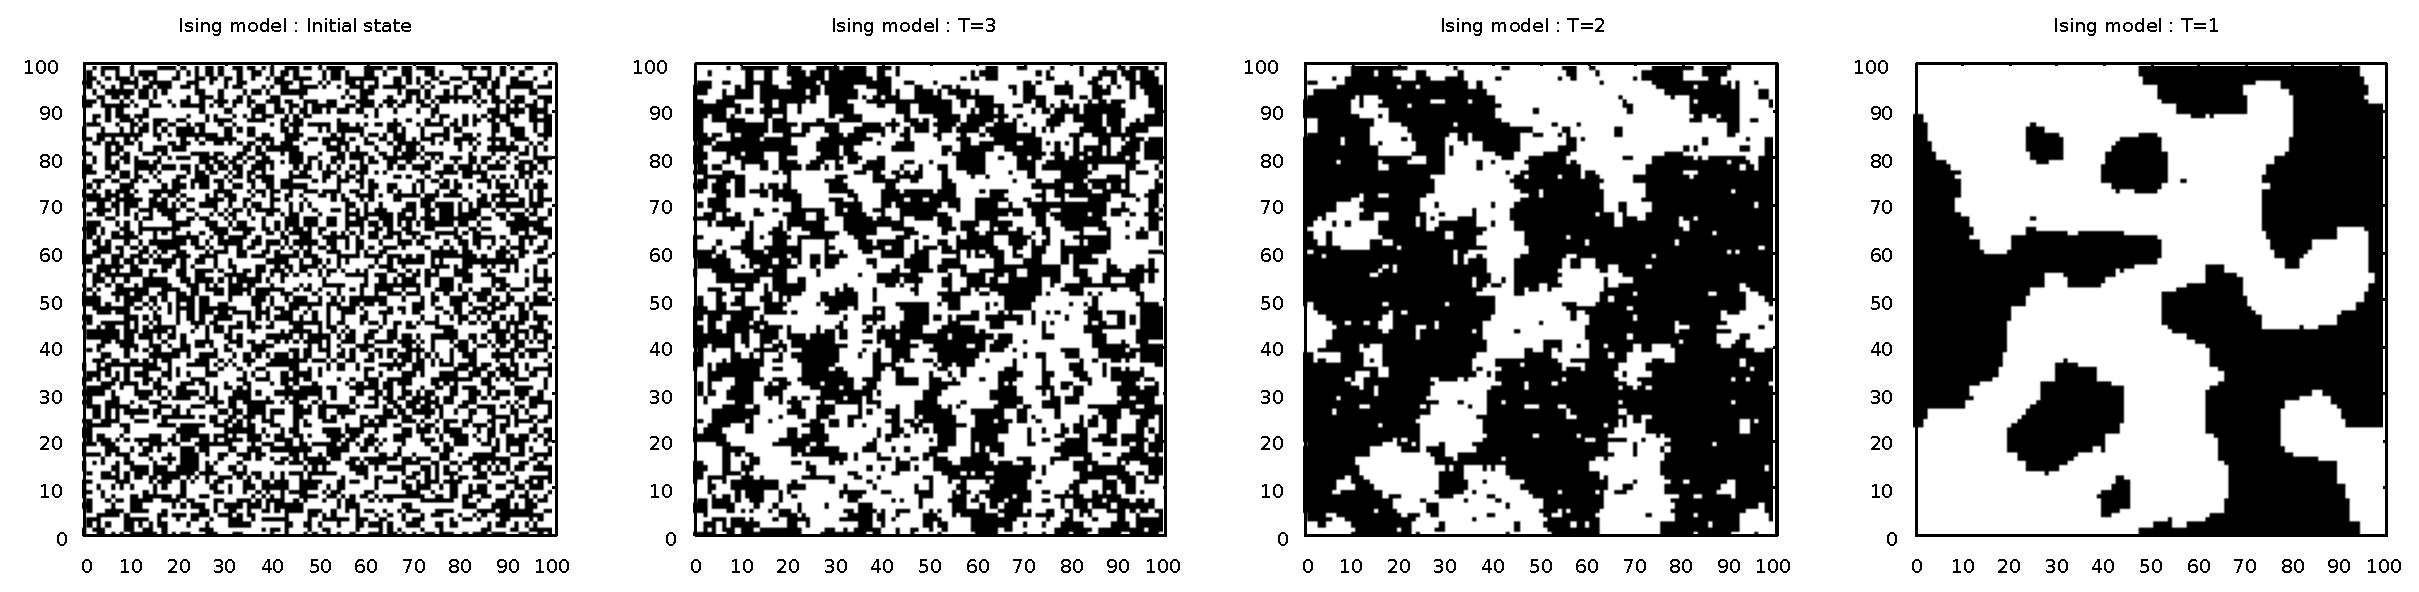
\includegraphics[width = 17cm]{./EPS/spin.eps}
  \end{center}
  \label{fig1}
\end{figure}\\
\begin{figure}[htbp]
  \begin{center}
    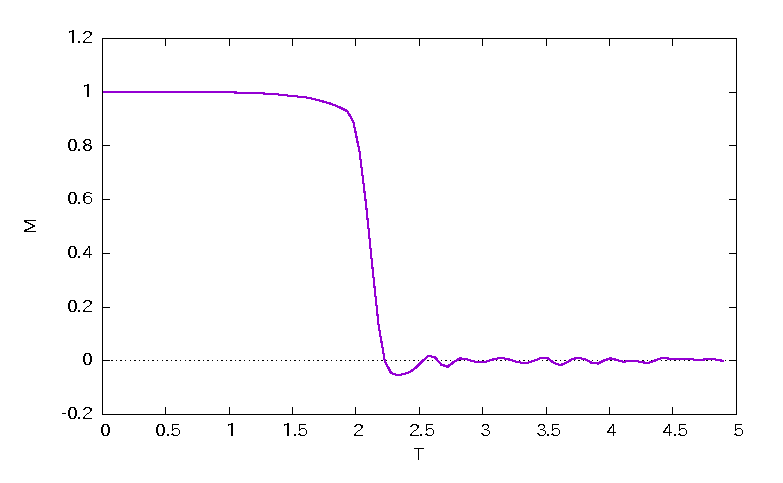
\includegraphics[width = 10cm]{./EPS/magnetization.eps}
  \end{center}
  \label{fig2}
\end{figure}\\
\begin{figure}[htbp]
  \begin{center}
    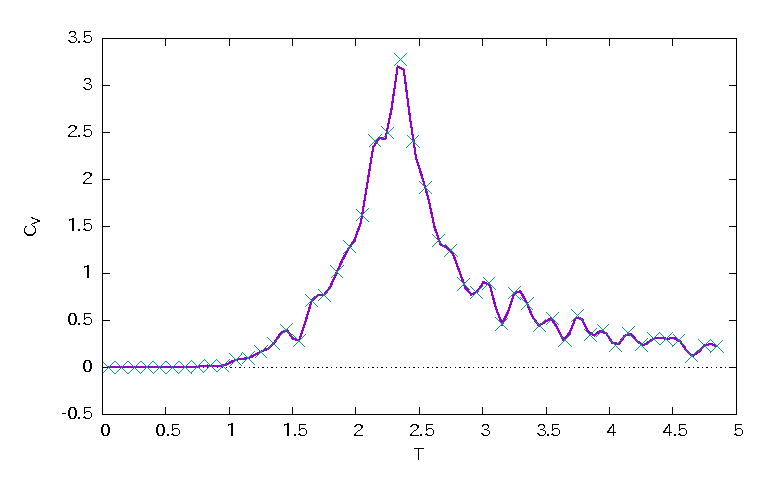
\includegraphics[width = 10cm]{./EPS/specificheat.eps}
  \end{center}
  \label{fig2}
\end{figure}\\

磁区の図は$N=100^2, J=1$, 磁化と比熱は$N=16^2, J=1$で計算した. 以上の図から
\begin{itemize}
\item 温度が下がるほどはっきりとした磁区が形成されること
\item 磁化・比熱は転移温度($T_C \simeq 2.26$)付近でdrasticに変化していること
\item 2次相転移が起こっている(であろう)こと
\end{itemize}
などがわかる.

\subsection{数値計算上の注意}
\subsubsection{乱数}
なるべく良い乱数を用いるようにしましょう. C言語のrand()はあまり良くありません. 単純な線形合同法では周期が短く大量の乱数を用いるシミュレーションには向きません. Mersenne twisterなどのアルゴリズムを用いましょう.
\subsubsection{ローカルな極小点}
ゼロ温度系ではあまり明確な磁区が生まれません. ただのMonte Carlo法ではローカルな極小点にハマるとそこから抜け出せないからです. Metropolis法を適応するとある程度解決しますが, やはり正の磁区と負の磁区に分かれるのでグローバルな磁化は熱力学極限とは異なる値を示します. 上の図の$T=1$もやはりローカルな極小点であり真の最小点であるスピンが全て揃った状態にはなりません. これを解決するために, 物理量の計算の際は$T=0$でスピンが全て揃った状態を用意しそこからMonte Carloシミュレーションを行っています. 焼きなまし法を用いるとどんな初期状態でもHelmholtzエネルギーが最小な状態を作れるかもしれません.
\begin{figure}[htbp]
  \begin{center}
    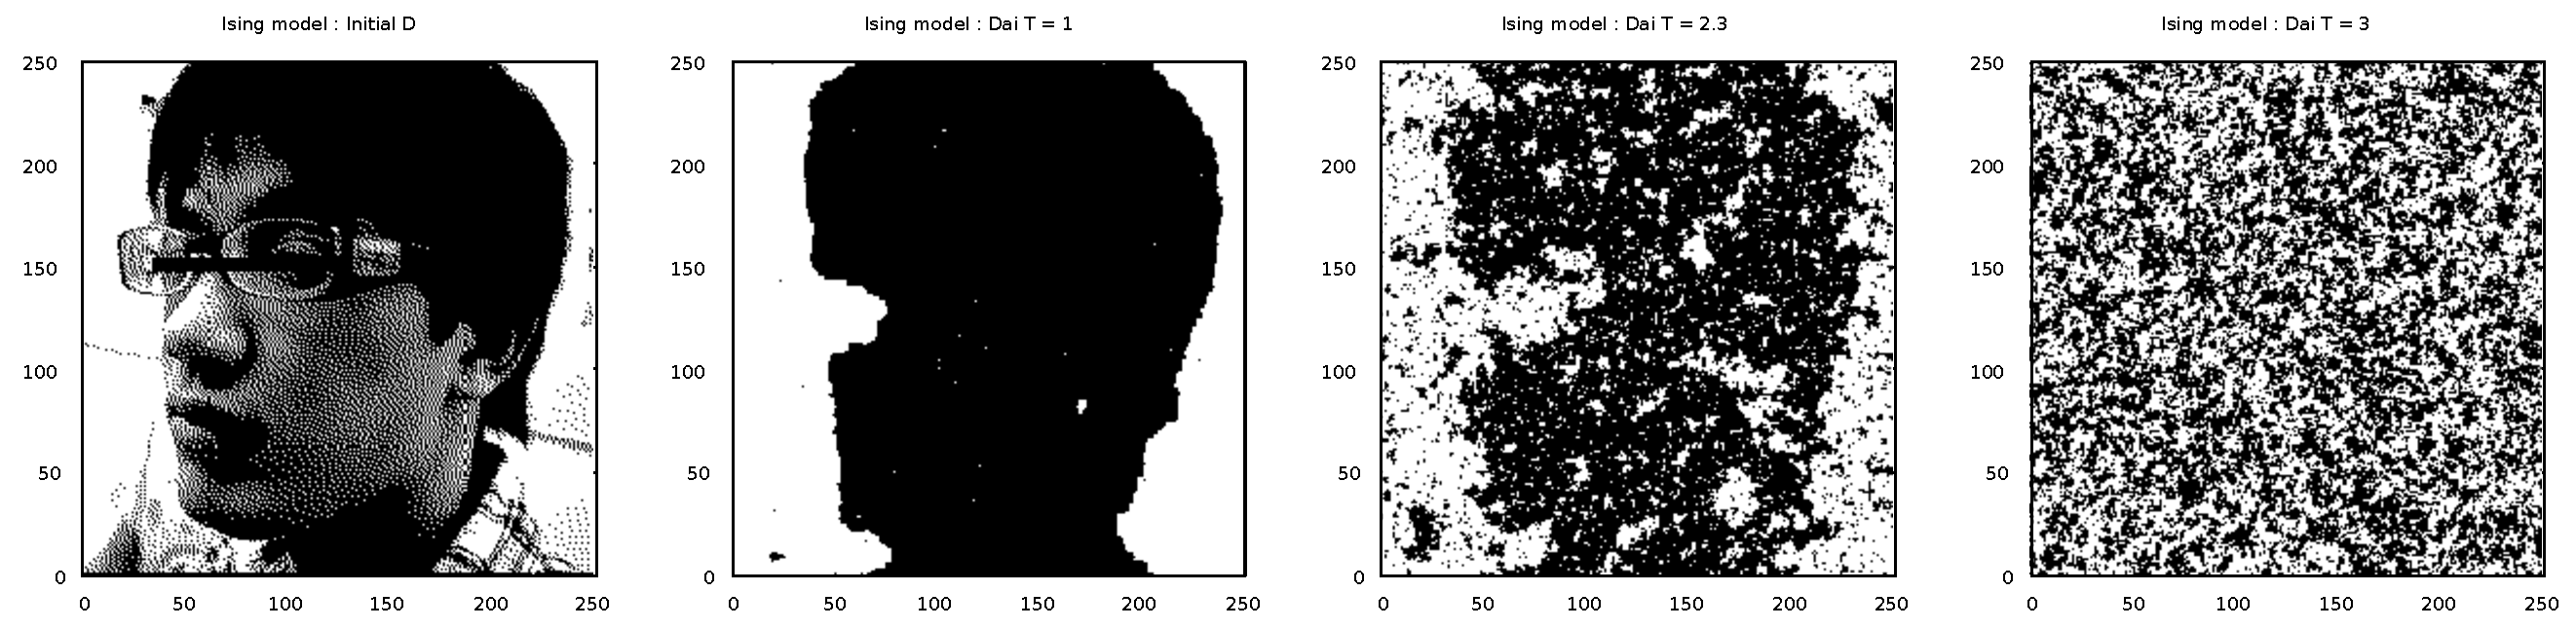
\includegraphics[width = 17cm]{./EPS/Dai.eps}
  \end{center}
  \label{Dai}
\end{figure}\\
ご覧の通り, Metropolis法だと磁化の形成は初期状態の選び方に強く依存します.


